% !TEX root = ./main.tex
\chapter{Impacts of emissions spatial heterogeneity on aerosol properties and CCN activity}
%\chapter{Impacts of emissions spatial heterogeneity on aerosol properties in a particle resolved framework}

\section{Ideal coagulation runs}


\section{Full multiphase chemistry runs}

\subsection{aerosol size distributions}
\begin{itemize}
\item Number dist \hl{render}
\item Mass dist \hl{render}
\end{itemize}

\subsection{aerosol composition}

\begin{itemize}
\item Time-height plots for sulfate, nitrate, ammonium
\item \% mass fraction vs particle diameter plots
\item kappa distributions (either here or in the ccn subsection?) \hl{render}
\end{itemize}

\subsection{aerosol mixing state}

\begin{itemize}
\item Vertical profile of average particle $\chi$, $D_{\alpha}$, $D_{\gamma}$
\item Vertical profile of ccn $\chi$, $D_{\alpha}$, $D_{\gamma}$
\end{itemize}

\subsection{ccn}

\begin{itemize}
\item Vertical profile of ccn conc at each supersaturation level
\item Vertical profile of ccn $\chi$, $D_{\alpha}$, $D_{\gamma}$
\item time height plots of ccn \% error
\item (potentially) some sort of box plot ccn error thing similar to what I showed at IAMA?
\end{itemize}

\subsection{Runs without ammonia}

\begin{itemize}
\item Vertical profile of SNA
\item Vertical profile of ccn conc at each supersaturation level
\end{itemize}

\newpage
\begin{figure}[h]
  \centering
    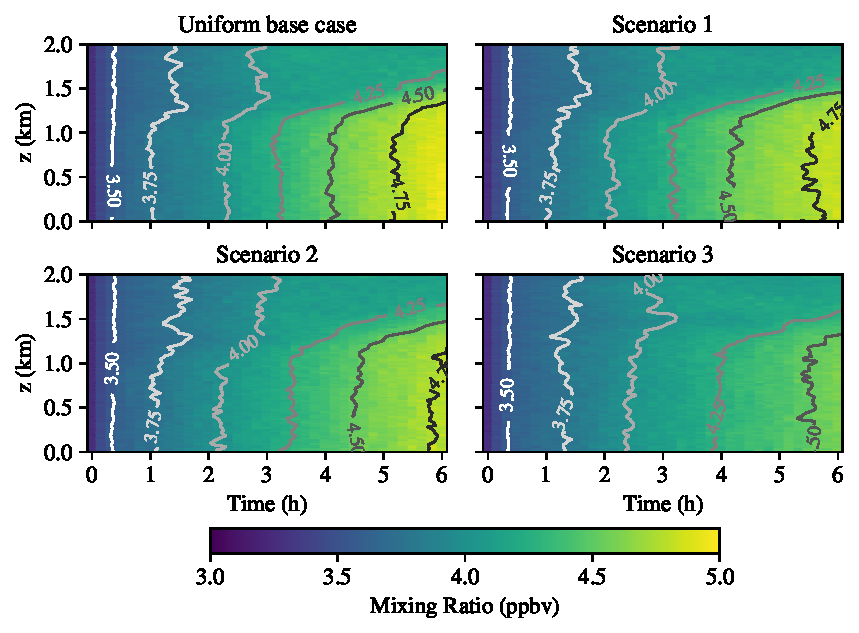
\includegraphics[width=\textwidth]{figures/chapter5/height-time-pmc_SO4-four-scenarios.pdf}
    \caption{Sulfate}
    \label{fig:ht-so4}
\end{figure}

\newpage
\begin{figure}[h]
  \centering
    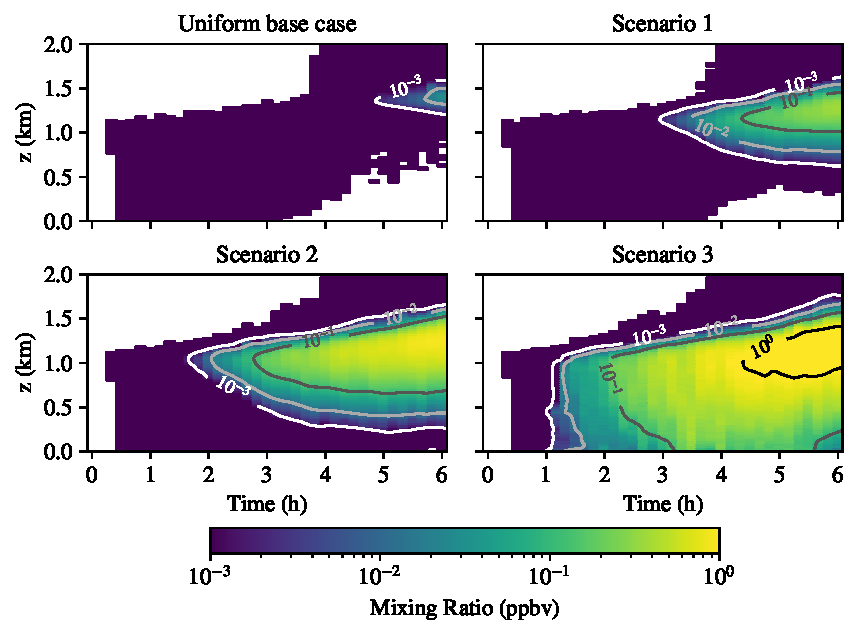
\includegraphics[width=\textwidth]{figures/chapter5/height-time-pmc_NO3-four-scenarios.pdf}
    \caption{Nitrate}
    \label{fig:ht-no3}
\end{figure}

\newpage
\begin{figure}[h]
  \centering
    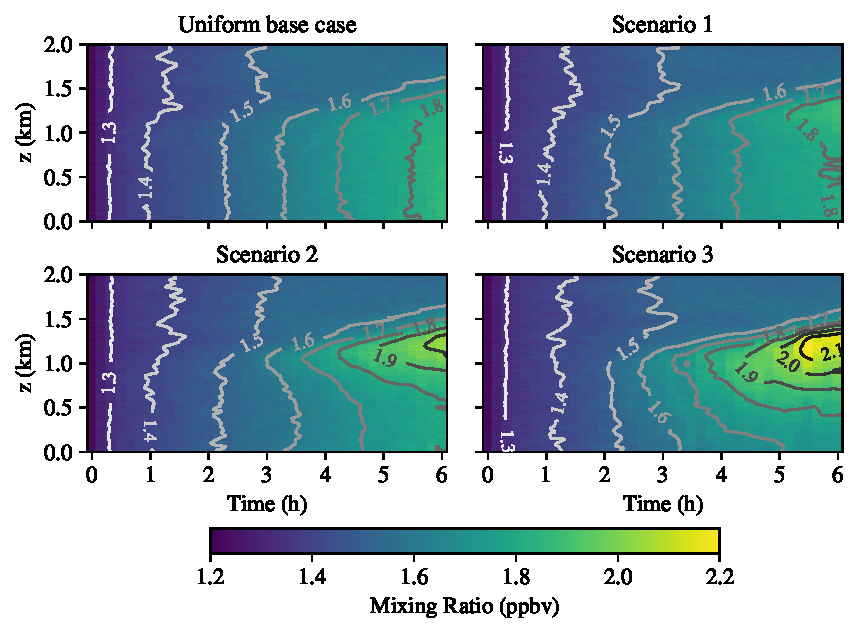
\includegraphics[width=\textwidth]{figures/chapter5/height-time-pmc_NH4-four-scenarios.pdf}
    \caption{Ammonium}
    \label{fig:ht-nh4}
\end{figure}


\newpage
\begin{figure}[h]
  \centering
    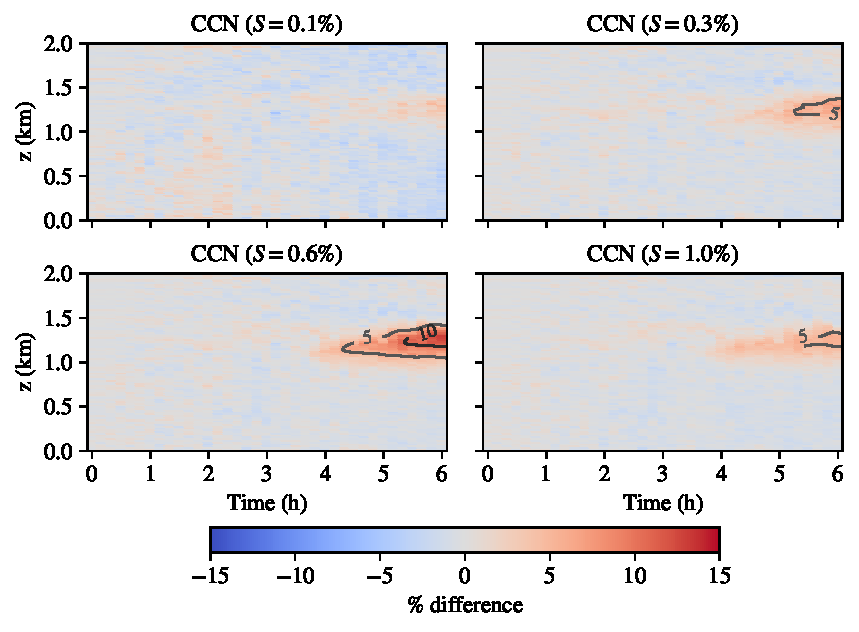
\includegraphics[width=\textwidth]{figures/chapter5/height-time-ccn-pdiff-fx1fy0.pdf}
    \caption{Scenario 1}
    \label{fig:ht-ccn-pdiff-s1}
\end{figure}

\newpage
\begin{figure}[h]
  \centering
    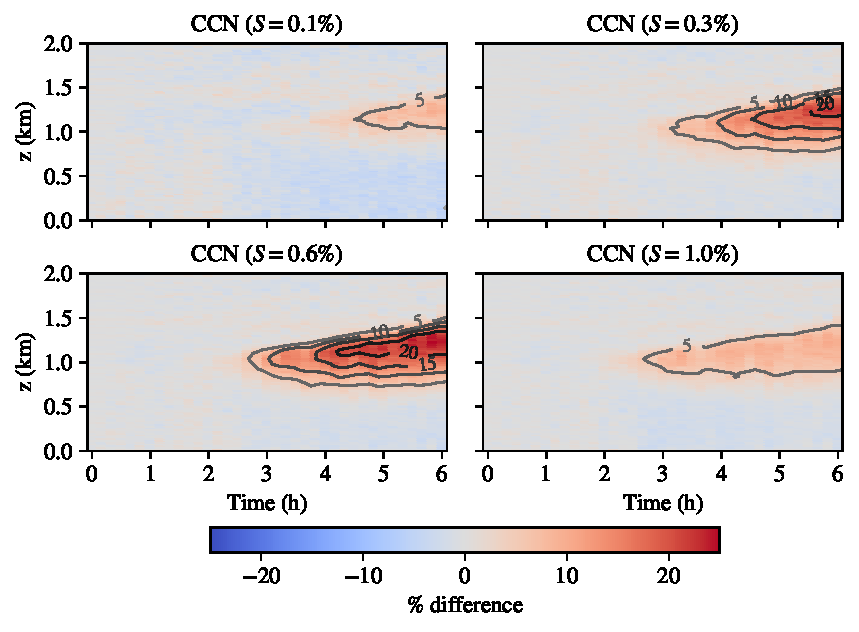
\includegraphics[width=\textwidth]{figures/chapter5/height-time-ccn-pdiff-road-10x.pdf}
    \caption{Scenario 2}
    \label{fig:ht-ccn-pdiff-s2}
\end{figure}

\newpage
\begin{figure}[h]
  \centering
    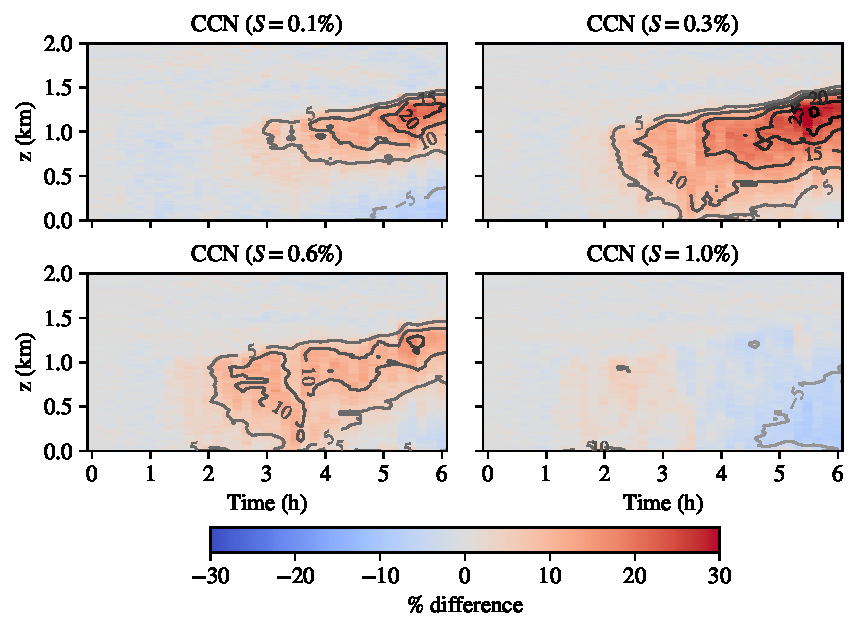
\includegraphics[width=\textwidth]{figures/chapter5/height-time-ccn-pdiff-point-source-1x1.pdf}
    \caption{Scenario 3}
    \label{fig:ht-ccn-pdiff-s3}
\end{figure}

